\documentclass[11pt]{beamer}
\usetheme{default}
\usefonttheme[onlymath]{serif}
\setbeamertemplate{navigation symbols}{}
\setbeamertemplate{footline}[frame number]
\setbeamertemplate{itemize items}[circle]
\setbeamertemplate{blocks}[rounded][shadow=false]
\definecolor{ink}{RGB}{28,42,80}
\definecolor{chalkblue}{RGB}{70,120,170}
\definecolor{chalkorange}{RGB}{205,120,50}
\setbeamercolor{structure}{fg=ink}
\setbeamercolor{block title}{bg=ink,fg=white}
\setbeamercolor{block body}{bg=ink!6}
\setbeamerfont{frametitle}{series=\bfseries,size=\large}
\setbeamerfont{block title}{series=\bfseries}
\setbeamerfont{title}{series=\bfseries,size=\LARGE}

% Build the speaker notes with crouzeix_talk_notes.tex, which defines \shownotes
% and inputs this file.
\ifdefined\shownotes
  \setbeameroption{show only notes}
  \setbeamerfont{note page}{size=\footnotesize}
\else
  \setbeameroption{hide notes}
\fi

\usepackage[T1]{fontenc}
\usepackage{lmodern}
\usepackage{amsmath,amssymb,mathtools}
\usepackage{tikz}
\usetikzlibrary{arrows.meta,calc}

\newcommand{\C}{\mathbb{C}}
\newcommand{\D}{\mathbb{D}}
\newcommand{\Hil}{\mathcal{H}}
\newcommand{\K}{\mathcal{K}}
\newcommand{\B}{\mathcal{B}}
\newcommand{\A}{\mathcal{A}}
\newcommand{\norm}[1]{\lVert #1\rVert}
\newcommand{\ip}[2]{\langle #1,#2\rangle}
\DeclareMathOperator{\re}{Re}
\DeclareMathOperator{\alg}{alg}
\DeclareMathOperator{\ran}{ran}
\DeclareMathOperator{\conv}{conv}

% Address of the interactive version; edit once the site is live.
\newcommand{\siteurl}{bnic101.github.io/crouzeix-folie-a-deux}

\title{Crouzeix: Folie \`a Deux}
\author{Nic Berkopec}
\date{October 2026}

\begin{document}

\begin{frame}
  \titlepage
  \begin{center}\small Interactive version: \texttt{\siteurl}\end{center}
\end{frame}
\note{
  [1 min.] A conjecture open since 2004, proved twice in the last week of July 2026, by two groups who did not know of each other, by two methods that turn out to be the same method. Both papers credit ChatGPT with the decisive idea; I will say exactly what the papers say about that, near the end, and no more. The title is a diagnosis: a shared delusion, two patients.

  The slides exist as a website with the pictures live; the address is on the title page.
}

%======================================================================
\begin{frame}{Numerical range}
  \textbf{Definition.} Let $\Hil$ be a complex Hilbert space and $T\in\B(\Hil)$ a bounded operator. The numerical range of $T$ is
  \[
    W(T)=\{\ip{Tx}{x}:\ x\in\Hil,\ \norm{x}=1\}.
  \]
  In finite dimension $W(T)$ is compact and convex (Toeplitz--Hausdorff); in general it is convex, and $\overline{W(T)}\supseteq\conv\sigma(T)$.

  \begin{center}
  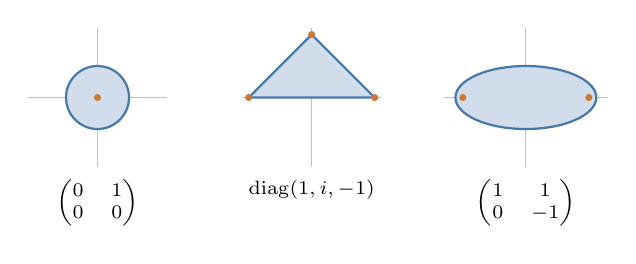
\begin{tikzpicture}[scale=0.8,>=Stealth]
    % nilpotent: disk of radius 1/2
    \begin{scope}[xshift=0cm]
      \draw[gray!50,thin] (-1.1,0)--(1.1,0) (0,-1.1)--(0,1.1);
      \fill[chalkblue!25] (0,0) circle (0.5);
      \draw[chalkblue,thick] (0,0) circle (0.5);
      \fill[chalkorange] (0,0) circle (1.6pt);
      \node[below,font=\scriptsize] at (0,-1.15) {$\begin{pmatrix}0&1\\0&0\end{pmatrix}$};
    \end{scope}
    % normal: triangle
    \begin{scope}[xshift=3.4cm]
      \draw[gray!50,thin] (-1.1,0)--(1.1,0) (0,-1.1)--(0,1.1);
      \fill[chalkblue!25] (1,0)--(0,1)--(-1,0)--cycle;
      \draw[chalkblue,thick] (1,0)--(0,1)--(-1,0)--cycle;
      \fill[chalkorange] (1,0) circle (1.6pt) (0,1) circle (1.6pt) (-1,0) circle (1.6pt);
      \node[below,font=\scriptsize] at (0,-1.15) {$\mathrm{diag}(1,i,-1)$};
    \end{scope}
    % 2x2 with ellipse, foci +-1
    \begin{scope}[xshift=6.8cm]
      \draw[gray!50,thin] (-1.3,0)--(1.3,0) (0,-1.1)--(0,1.1);
      \fill[chalkblue!25] (0,0) ellipse (1.118 and 0.5);
      \draw[chalkblue,thick] (0,0) ellipse (1.118 and 0.5);
      \fill[chalkorange] (1,0) circle (1.6pt) (-1,0) circle (1.6pt);
      \node[below,font=\scriptsize] at (0,-1.15) {$\begin{pmatrix}1&1\\0&-1\end{pmatrix}$};
    \end{scope}
  \end{tikzpicture}
  \end{center}
  \vspace{-4pt}
  {\footnotesize Orange: spectrum. Blue: numerical range. A normal operator has $\overline{W(T)}=\conv\sigma(T)$; a $2\times2$ matrix has an ellipse with foci at the eigenvalues.}
\end{frame}
\note{
  [3 min.] The numerical range is convex, contains the spectrum in its closure, and for normal operators is exactly the convex hull of the spectrum. The three pictures are the whole zoo for this talk: the nilpotent, whose numerical range is a disk of radius one half around the single eigenvalue; a normal matrix, a triangle; and a general $2\times2$, an ellipse with the eigenvalues as foci. For a $2\times2$ matrix the minor axis is $|t_{12}|$ in Schur form.

  On the website you can pick these and other examples and see the eigenvalues, the numerical range and the numerical radius.
}

%======================================================================
\begin{frame}{Spectral sets}
  \textbf{Definition.} A compact set $S\subset\C$ is a \emph{$K$-spectral set} for $T\in\B(\Hil)$ if
  \[
    \norm{p(T)}\le K\sup_{z\in S}|p(z)|\qquad\text{for all } p\in\C[z].
  \]
  (For convex $S$, functions holomorphic near $S$ come along by Runge.)

  \medskip
  \textbf{von Neumann's inequality (1951).} The closed disk is a spectral set for every contraction:
  \[
    \norm{T}\le1\ \Rightarrow\ \norm{p(T)}\le\sup_{\D}|p|.
  \]
  Also the closed right half-plane, when $\re T\ge0$.

  \medskip
  Two proofs:
  \begin{itemize}
    \item \textbf{Function theory.} von Neumann: reduce to Blaschke products, check M\"obius maps by hand.
    \item \textbf{Dilation theory.} Sz.-Nagy: $T$ is the compression of a unitary $U$, and $p(T)=P_\Hil\,p(U)|_\Hil$.
  \end{itemize}
\end{frame}
\note{
  [3 min.] Spectral set is von Neumann's word, and his inequality is the model result. There are two classical proofs and they are the two themes of this talk. von Neumann proved it by function theory: reduce to Blaschke products, which are compositions of M\"obius maps, and check the M\"obius case by hand. Sz.-Nagy proved it by dilation: every contraction is the compression of a unitary, and the functional calculus of a unitary is bounded by the sup norm on the circle.

  The two 2026 proofs of Crouzeix are, respectively, a function-theory proof and a dilation-theory proof. Keep the pairing in mind.
}

%======================================================================
\begin{frame}{Crouzeix's conjecture}
  \begin{block}{Conjecture (Crouzeix 2004)}
    Let $T$ be a bounded operator on a Hilbert space $\Hil$. Then $\overline{W(T)}$ is a $2$-spectral set for $T$.
  \end{block}

  \medskip
  \textbf{Remark.} The constant is sharp. For $N=\begin{pmatrix}0&1\\0&0\end{pmatrix}$ and $p(z)=z$,
  \[
    W(N)=D(0,\tfrac12),\qquad \norm{p(N)}=1=2\cdot\tfrac12=2\sup_{D(0,1/2)}|p|.
  \]

  \medskip
  \textbf{Antecedents.}
  \begin{itemize}
    \item von Neumann: constant $1$, only for contractions.
    \item Berger 1965, Berger--Stampfli 1967, Okubo--Ando 1975: the disk is a $2$-spectral set whenever it contains $W(T)$. Via $2$-dilations: $T^n=2V^*U^nV$.
  \end{itemize}
  So Crouzeix asks for the disk's constant on every convex set. For $2\times2$ matrices he proved it, with equality only when $W(T)$ is a disk.
\end{frame}
\note{
  [3 min.] The statement, the example, and the antecedents. $\ip{Nx}{x}=x_2\bar x_1$ has modulus at most $\frac12$, with every value in that disk attained, while $\norm N=1$. So nothing below $2$ can work.

  For the disk the constant $2$ is classical and comes from dilation theory: Berger showed numerical radius at most one is the same as having a $2$-dilation, and Okubo--Ando turned that into the bound for all polynomials. The conjecture says the disk is the worst convex set. Crouzeix checked it for $2\times2$ matrices, where the exact constant is a function of the eccentricity of the ellipse.
}

%======================================================================
\begin{frame}{Constants}
  $\Omega$ bounded convex with smooth boundary, $W(T)\subset\Omega$; $A(\Omega)$ the functions holomorphic on $\Omega$, continuous on $\overline\Omega$.
  \[
    C_\Omega:=\sup\big\{\norm{f(T)}:\ W(T)\subset\Omega,\ \norm{f}_\infty\le1\big\}.
  \]
  {\footnotesize
  \begin{tabular}{@{}llll@{}}
    Delyon--Delyon & 1999 & $C_\Omega<\infty$ & depends on $\Omega$\\
    Crouzeix & 2004 & $2$ & only for $2\times2$\\
    Crouzeix & 2007 & $11.08$ & uniform in $\Omega$\\
    Crouzeix--Palencia & 2017 & $1+\sqrt2$ & completely bounded\\
    Jin & 27 July 2026 & $2$ & function theory\\
    Lorist--Schwenninger & Aug 2026 & $2$ & dilation theory
  \end{tabular}}

  \medskip
  \textbf{Technique}, 1999 to 2026: one object, the double-layer potential. Shrinking $\Omega$ to $\overline{W(T)}$, $\sup_\Omega C_\Omega\le2$ is the conjecture.
\end{frame}
\note{
  [2 min.] From here on $\Omega$ is a smooth bounded convex domain strictly containing the numerical range. Delyon--Delyon introduced the double-layer potential and got a constant depending on the shape. Crouzeix 2007 got a universal $11.08$ by estimating the Cauchy transform hard. Crouzeix--Palencia got $1+\sqrt2$ in six pages, and the argument survives matrix-valued $f$. Nine years, then two proofs within a week.
}

%======================================================================
\begin{frame}{Double-layer potential}
  For $\sigma\in\partial\Omega$ let $\nu=\nu(\sigma)$ be the outward unit normal and $ds$ arclength. For $z\in\Omega$,
  \[
    \mu(\sigma,z)=\frac{1}{2\pi}\Big(\underbrace{\frac{\nu}{\sigma-z}}_{\text{first layer}}+\underbrace{\frac{\bar\nu}{\bar\sigma-\bar z}}_{\text{second layer}}\Big)
    =\frac1\pi\re\frac{\nu}{\sigma-z}.
  \]
  \begin{columns}[T]
  \begin{column}{0.48\textwidth}
    \begin{center}
    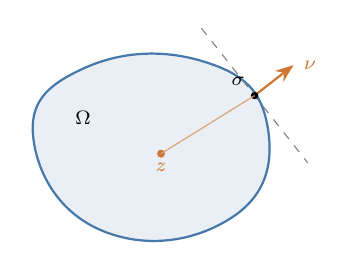
\begin{tikzpicture}[scale=0.9,>=Stealth]
      \fill[chalkblue!12] plot[smooth cycle,tension=0.8] coordinates {(-1.6,0.1) (-0.9,1.1) (0.8,1.2) (1.7,0.3) (1.2,-1.0) (-0.6,-1.2)};
      \draw[chalkblue,thick] plot[smooth cycle,tension=0.8] coordinates {(-1.6,0.1) (-0.9,1.1) (0.8,1.2) (1.7,0.3) (1.2,-1.0) (-0.6,-1.2)};
      \coordinate (s) at (1.52,0.72);
      \draw[gray,dashed] ($(s)+(-0.75,0.95)$) -- ($(s)+(0.75,-0.95)$);
      \draw[chalkorange,thick,->] (s) -- ++(0.55,0.43) node[right,font=\scriptsize] {$\nu$};
      \fill (s) circle (1.5pt) node[above left,font=\scriptsize] {$\sigma$};
      \fill[chalkorange] (0.2,-0.1) circle (1.6pt) node[below,font=\scriptsize] {$z$};
      \draw[chalkorange!70] (0.2,-0.1) -- (s);
      \node[font=\scriptsize] at (-0.9,0.4) {$\Omega$};
    \end{tikzpicture}
    \end{center}
  \end{column}
  \begin{column}{0.52\textwidth}
    \small
    \begin{itemize}
      \item First layer: the Cauchy kernel, $\frac{1}{2\pi}\frac{\nu\,ds}{\sigma-z}=\frac{1}{2\pi i}\frac{d\sigma}{\sigma-z}$.
      \item $\mu\,ds=\frac1\pi\,d\arg(\sigma-z)$: the angle at which $z$ sees the boundary. So $\mu\ge0$ by convexity, and $\int\mu\,ds=2$ for $z\in\Omega$, $1$ for $z\in\partial\Omega$.
      \item Why use it? The first layer gives $f(z)$. If we can control the second layer, we win.
    \end{itemize}
  \end{column}
  \end{columns}
\end{frame}
\note{
  [4 min.] The kernel is twice the real part of the Cauchy kernel. The scalar picture: $\mu\,ds$ is the angle subtended at $z$ by a piece of boundary, divided by $\pi$. So it is positive by convexity, since $z$ sits on the inner side of every tangent line, and it integrates to $2$ going once round. On the boundary it integrates to $1$; the jump in between is the Gauss jump relation, which is what makes the Cauchy transform of $\bar f$ continuous up to the boundary.

  On the website: drag $z$ and watch the density on the boundary and its integral. Push $z$ to the boundary and watch half the mass collapse onto the nearest point.

  Why bother? Because the first layer alone is Cauchy's formula. The second layer is the price of positivity.
}

%======================================================================
\begin{frame}{Double-layer potential, continued}
  Replace $z$ by $T$ with $W(T)\subset\Omega$. For $f\in C(\partial\Omega)$ put
  \[
    C(f,T)=\frac{1}{2\pi i}\int_{\partial\Omega}f(\sigma)(\sigma-T)^{-1}\,d\sigma,
  \]
  \[
    S(f,T)=C(f,T)+C(\bar f,T)^*.
  \]
  $S$ is the functional calculus integrated against the double-layer potential
  $\mu(\sigma,T)=\tfrac1\pi\re[\nu(\sigma)(\sigma-T)^{-1}]$:
  \[
    S(f,T)=\int_{\partial\Omega}f(\sigma)\,\mu(\sigma,T)\,ds,
    \qquad \mu(\sigma,T)\ge0,\qquad \int_{\partial\Omega}\mu\,ds=2I.
  \]
  \begin{lemma}[Crouzeix--Palencia 2017]
    For $f\in A(\Omega)$,\quad $\norm{S(f,T)}=\norm{f(T)+C(\bar f,T)^*}\le2\norm{f}_{\partial\Omega}$.
  \end{lemma}
  Positivity and total mass $2I$, then Cauchy--Schwarz.

  \medskip
  So the question: how does $\norm{S(f,T)}$ control $\norm{f(T)}$? Can we estimate $C(\bar f,T)^*$, or make it vanish altogether?
\end{frame}
\note{
  [3 min.] Positivity transfers: $\ip{Tx}{x}\in\Omega$ for unit $x$ gives $\re\,\bar\nu(\sigma-T)\ge0$, and conjugating by the resolvent gives $\mu(\sigma,T)\ge0$. Total mass $2I$ is Cauchy's formula for the first layer plus its adjoint.

  For holomorphic $f$ the first layer is $f(T)$. The second layer is the adjoint of the Cauchy integral of $\bar f$, not of $f$, because the conjugation falls on $f$ as well as on the kernel. So positivity bounds $f(T)$ plus a companion. The companion is the whole subject.
}

%======================================================================
\begin{frame}{Positivity and the double-layer formula}
  Write $\Phi(f)=\tfrac12S(f,T)$, a unital positive map $C(\partial\Omega)\to\B(\Hil)$. For $f\in A(\Omega)$,
  \[
    2\Phi(f)=f(T)+\alpha(f)(T)^*,\qquad
    \alpha(f)(z)=\frac{1}{2\pi i}\int_{\partial\Omega}\frac{\overline{f(\sigma)}\,d\sigma}{\sigma-z},
  \]
  where $\alpha:A(\Omega)\to A(\Omega)$ is antilinear and $\alpha(1)=1$. Positivity of $\Phi$ is the lemma: $\norm{2\Phi(f)}\le2\norm{f}$.

  \medskip
  For a point $z$ this is $2\Phi(f)(z)=f(z)+\overline{\alpha(f)(z)}$: the weighted average of $f$ on the boundary, split into a holomorphic and an anti-holomorphic piece. For the disk, $\alpha(f)=\overline{f(0)}$, a constant.

  \medskip
  \textbf{Two ways to use the formula.}
  \begin{itemize}
    \item Estimate the companion: Crouzeix--Palencia, $\norm{\alpha(f)}\le\norm f$, hence $1+\sqrt2$.
    \item Study the extremal $f$, a Blaschke product, and show $\norm{f(T)}\le\norm{2\Phi(f)}$ for it: Bickel, Gorkin, Greenbaum, Overton. Not the route either 2026 proof takes.
  \end{itemize}
\end{frame}
\note{
  [3 min.] Same identity, with $\Phi$ for half of $S$ and $\alpha$ for the Cauchy transform of the conjugate. Two things to say.

  Scalar picture: for a point, the right side is harmonic, holomorphic plus anti-holomorphic, and the identity says which anti-holomorphic function completes $f$ to the double-layer potential of its own boundary values. The website shows the two vectors adding. For the disk the companion is the constant $\overline{f(0)}$, which is why the disk is easy: Berger--Stampfli is the identity read off directly.

  Two programmes grew from this. Crouzeix--Palencia estimate the companion's size. Bickel, Gorkin and collaborators attack the extremal functions, which Crouzeix showed are Blaschke products. Neither 2026 proof uses the extremal functions at all.
}

%======================================================================
\begin{frame}{Crouzeix--Palencia: $1+\sqrt2$, and why not $2$}
  Let $K=C_\Omega$, $\norm{f}\le1$, $T=f(A)$, $g=\alpha(f)$. Since $\norm{g}\le\norm{f}$ on convex $\Omega$,
  \[
    TT^*TT^*=T\,\big(T+g(A)^*\big)^*\,TT^*-(fgf)(A)\,T^*,
  \]
  so $K^4\le2K^3+K^2$ and $K\le1+\sqrt2$. \hfill(Ransford--Schwenninger's four lines)

  \medskip
  Only two facts about the companion were used: $\norm{f(A)+g(A)^*}\le2$ and $\norm g\le\norm f$. Under those two alone, $1+\sqrt2$ is attained:
  $T=\begin{pmatrix}1&1\\0&0\end{pmatrix}$, $\Omega$ two small disks about $0$ and $1$, $g=-f(0)$ on one, $-f(1)$ on the other, $h=\mp1$ gives $\norm{h(T)}=1+\sqrt2$.

  \medskip
  Not a counterexample, since $W(T)\not\subset\Omega$, but the end of that road. This $g$ sends $1\mapsto-1$; the Cauchy transform sends $1\mapsto1$.
\end{frame}
\note{
  [4 min.] Replace the middle $T^*$ in $TT^*TT^*$ by $(T+g(A)^*)^*-g(A)$. The first piece contains $T+g(A)^*$, norm at most $2$; the second is $(fgf)(A)$, and $fgf$ has sup norm at most $1$ by the lemma. Hence $K^4\le2K^3+K^2$.

  Ransford and Schwenninger showed this is sharp for the information used: with $T^n=T$, $f(T)=\begin{pmatrix}f(1)&f(1)-f(0)\\0&f(0)\end{pmatrix}$, the ad hoc $g$ satisfies both estimates, and $h(T)=\begin{pmatrix}1&2\\0&-1\end{pmatrix}$ has norm $1+\sqrt2$. The extra information available and not yet used is that the Cauchy transform is unital.
}

%======================================================================
\begin{frame}{Equivalent formulation}
  \begin{theorem}[Twisted real part]
    Let $\A$ be a unital commutative operator algebra, $\theta:\A\to\B(\Hil)$ a unital bounded homomorphism, and $\alpha:\A\to\A$ a unital antilinear map such that the unital linear map
    \[
      \theta_\alpha:\A\to\B(\Hil),\qquad a\mapsto\tfrac12\big(\theta(a)+\theta(\alpha(a))^*\big)
    \]
    is contractive. Then $\norm{\theta}\le2$.
  \end{theorem}
  \begin{itemize}
    \item Ransford--Schwenninger (2018) and Clou\^atre--Ostermann--Ransford (2023): this statement implies Crouzeix. Take $\theta(f)=f(T)$, $\alpha$ the Cauchy transform; then $\theta_\alpha=\Phi$.
    \item Michael Hartz (31 July 2026) proves the theorem, by reorganising Jin's solution.
  \end{itemize}
  \medskip
  Unital and contractive implies positive: $\re a\ge0\Rightarrow\re\theta_\alpha(a)\ge0$. The hypothesis is positivity of the twisted real part.
\end{frame}
\note{
  [2 min.] The abstract question, now a theorem. The numerical range and the Cauchy transform are gone; what remains is a homomorphism, a unital antilinear twist, and positivity of the symmetrised map. In the application $\theta_\alpha=\Phi$. Both 2026 proofs establish this, Hartz's version exactly as stated, Lorist--Schwenninger's with ``contractive'' strengthened to ``completely positive'', which costs nothing here because $\Phi$ lives on a commutative $C^*$-algebra.
}

%======================================================================
\begin{frame}
  \begin{center}
    {\Large\itshape Un}\\[6pt]
    {\LARGE\bfseries Function theory}\\[12pt]
    {\small Jin, 27 July 2026. Operator form: Hartz, unpublished notes, 31 July 2026.}
  \end{center}
\end{frame}
\note{[0.5 min.] First proof: function theory. Carath\'eodory functions, a vector-valued Hardy space, one reproducing kernel.}

%======================================================================
\begin{frame}{Holomorphic $\to$ resolvent transfer}
  \begin{theorem}[Holomorphic $\to$ resolvent transfer; Jin, operator form Hartz]
    Let $T\in\B(\Hil)$ with $\sigma(T)\subset\overline\D$. Let $H:\D\to\B(\Hil)$ be holomorphic with $H(0)=I$ and $\re H(z)\ge0$ for all $z\in\D$. Assume that
    \[
      \Delta(z):=H(z)-(I-zT)^{-1}
    \]
    commutes with $T^*$ for all $z\in\D$. Then $\norm{T}\le2$.
  \end{theorem}
  \begin{itemize}
    \item $\Delta=0$: $\re(I-zT)^{-1}\ge0$ is Berger's condition $W(T)\subset\overline\D$, and the conclusion is Okubo--Ando. A commuting correction costs nothing.
    \item Transfer $\Rightarrow$ twisted real part (Hartz). $T=\theta(a)$, $c_z=(1+za)(1-za)^{-1}$, $H(z)=\theta_\alpha(c_z)$. Then $\re H\ge0$ and
      $\Delta(z)=\tfrac12(\theta(\alpha(c_z))^*-I)$, an adjoint from the commutative algebra $\theta(\A)\ni T$.
      Concretely $\Delta(w)=\sum_{m\ge1}w^m\alpha(f^m)(T)^*$: every power of $f$ at once.
  \end{itemize}
\end{frame}
\note{
  [4 min.] Read the theorem slowly. $H$ is an operator-valued Carath\'eodory function normalised at $0$; the resolvent is what $H$ would be if $T$ were well behaved; the hypothesis is that the defect is algebraically tame.

  Calibration: $\re(I-zT)^{-1}\ge0$ characterises the class $C_2$, so with no defect the theorem is Okubo--Ando.

  The transfer: the Cayley transform of a norm-one element has positive real part, a unital contraction preserves that, and the homomorphism property turns half of $\theta_\alpha(c_z)$ into the resolvent. The other half is an adjoint from the commutative algebra, so it commutes with $T^*$. In the Crouzeix setting, expanding the Cayley transform gives the double-layer identity for all powers $f^m$ simultaneously. Crouzeix--Palencia used it once.
}

%======================================================================
\begin{frame}{Proof of the transfer theorem}
  On $H^2\otimes\Hil$ (after scaling $T\to rT$), $\re M_H\ge0$ and $M_H=M_R+M_\Delta$, $R(z)=(I-zT)^{-1}$.

  \medskip
  For $W$ with $\sigma(W)\subset\D$ let $N_W=\{F=\sum F_nz^n:\ \sum W^nF_n=0\}$, the functions vanishing at $W$.
  \begin{itemize}
    \item $\Delta(z)$ commutes with $W$ $\Rightarrow$ $M_\Delta N_W\subset N_W$ (an ideal, as in one variable).
    \item $\Delta(0)=0$ $\Rightarrow$ the kernel $\Gamma$ of $N_W$ at $0$ has $\Gamma^*M_\Delta\Gamma=0$.
  \end{itemize}
  Take $W=\tfrac12T^*$:\quad $\Gamma^*(M_R+M_R^*)\Gamma=\Gamma^*(M_H+M_H^*)\Gamma\ge0$.

  \medskip
  Unwinding, with $P=\sum4^{-n}T^{*n}T^n$, $Q=\sum2^{-n}T^{*n}T^n$, $Y=Q-P\ge\tfrac14T^*T$:
  \[
    4Y-YP-PY\ge0\ \Rightarrow\ P\le2I\ \Rightarrow\ T^*T\le T^*PT=4(P-I)\le4I .
  \]
  Jin's coordinates: sample the Herglotz kernel of $H$ at $\lambda_i/2$ and at $0$, the origin vector chosen to cancel the diagonal correction. Same compression.
\end{frame}
\note{
  [4 min.] Positivity of $H$ is an operator inequality on the Hardy space. Compress to a subspace on which the defect is invisible: functions vanishing at the operator point $W$, which $M_\Delta$ preserves because $\Delta$ commutes with $W$, and whose kernel at the origin kills $M_\Delta$ because $\Delta(0)=0$. Evaluate at half the adjoint. The defect is removed exactly, never estimated.

  Then compute $\Gamma$; the resolvent identity produces two weighted Gramians with weights $4^{-n}$ and $2^{-n}$, the squares of the sampling radius. Their difference is positive, which makes an eigenvector argument give $P\le2I$, and the Stein identity $P=I+\frac14T^*PT$ finishes. Details in the appendix.
}

%======================================================================
\begin{frame}
  \begin{center}
    {\Large\itshape Deux}\\[6pt]
    {\LARGE\bfseries Dilation theory}\\[12pt]
    {\small Lorist and Schwenninger, arXiv 2608.03841, August 2026.}
  \end{center}
\end{frame}
\note{[0.5 min.] Second proof: dilation theory. Three pages. Okubo--Ando with an error term.}

%======================================================================
\begin{frame}{Dilation theory}
  \begin{lemma}[Lorist--Schwenninger]
    Let $\Hil$ be a Hilbert space and $T\in\B(\Hil)$. Suppose there exist a Hilbert space $\K$, a contraction $Q\in\B(\K)$ and an isometry $V\in\B(\Hil,\K)$ such that the operators
    \[
      E_n:=2V^*Q^{*n}V-T^{*n},\qquad n\in\mathbb N,
    \]
    are uniformly bounded and commute with $T$. Then $\norm{T}\le2$.
  \end{lemma}
  $E_n=0$: $T^*$ has a $2$-dilation and $\norm T=\norm{2V^*QV}\le2$ at once. The lemma tolerates an error of any size, if bounded in $n$ and commuting with $T$.

  \medskip
  The dilation is Stinespring for $\Phi$: $\K=L^2(\partial\Omega,ds;\Hil)$, $Vx=\tfrac1{\sqrt2}\mu(\cdot,T)^{1/2}x$, $Q=M_f$ with $\norm f_\infty=1$. Then $V^*Q^nV=\Phi(f^n)$, and with $T=f(A)$,
  $E_n=2\Phi(f^n)^*-f(A)^{*n}=\alpha(f^n)(A)$, which commutes with $f(A)$ and is bounded by $\norm\theta\norm\alpha$. Hence $\norm{f(A)}\le2$.
\end{frame}
\note{
  [4 min.] There is a genuine dilation here, of the positive map $\Phi$, not of $f(A)$. $V$ is an isometry precisely because $\Phi(1)=I$. Compressing the powers of the normal contraction $M_f$ gives $\Phi(f^n)$, and the double-layer identity for $f^n$ says the powers of $f(A)$ are those compressions, times $2$, up to the companion. So $f(A)$ has a perturbed $2$-dilation with error exactly the companion $\alpha(f^n)(A)$.

  The error commutes with $f(A)$ because both come from the same functional calculus, and it is bounded because $\alpha$ is bounded; Crouzeix had $9.08$ in 2007. The contractivity $\norm\alpha\le1$ is never used.
}

%======================================================================
\begin{frame}{Proof of the lemma}
  $\kappa:=\norm{T}>1$ and $x$ a unit vector with $T^*Tx=\kappa^2x$ (ultrapower if necessary). Put
  \[
    m_n:=\re\ip{E_nT^nx}{x},\qquad u:=Q^*VTx-\kappa Vx .
  \]
  Two estimates on the same error vector:
  \begin{align*}
    \norm{u}^2&\le 2\kappa^2-\kappa^3-\kappa m_1 && \text{($V$ isometric, $Q$ contractive, $n=1$ only)}\\[2pt]
    \kappa m_1&\ge-\frac{\norm{u}^2}{(\kappa-1)^2} && \text{(telescope $\kappa m_n-m_{n+1}$ over all $n$)}
  \end{align*}
  Together, $\norm{u}^2\big(1-(\kappa-1)^{-2}\big)\le\kappa^2(2-\kappa)$: impossible if $\kappa>2$.

  \bigskip
  The first line alone gives $\kappa\le1+\sqrt{1-m_1}$; with $\norm\alpha\le1$, $m_1\ge-1$, and that is $1+\sqrt2$ again. $m_1<0$ happens for some $3\times3$ matrices. The second line needs $E_n$ for every $n$.
\end{frame}
\note{
  [4 min.] The vector $u$ measures how far $VTx$ is from an eigenvector of $Q^*$ with the eigenvalue it would have if the dilation were exact. The upper bound uses the identity for $n=1$ only, and the quantity $m_1=\re\ip{(f\alpha(f))(A)x}{x}$ is the one central since Crouzeix--Palencia. The lower bound is new: a uniform bound on $\kappa m_n-m_{n+1}$ using the commutation, summed with weights $\kappa^{-n+1}$, telescoping to $\kappa m_1$. If $m_1\ge0$ were true in general the first line would finish; it is not, so the second line is not a luxury. Details in the appendix.
}

%======================================================================
\begin{frame}{The same proof twice}
  \small
  \begin{tabular}{@{}lll@{}}
     & Un (Jin, Hartz) & Deux (Lorist--Schw.)\\
    \hline\\[-8pt]
    positivity & $\re H\ge0$ & $\Phi=V^*\pi(\cdot)V$\\[2pt]
    all powers & $H(w)=I+2\sum_m w^m\Phi(f^m)$ & $E_n$, every $n$\\[2pt]
    companion & $\Delta(w)=\sum_m w^m\alpha(f^m)(T)^*$ & $E_n=\alpha(f^n)(T)$\\[2pt]
    used & commutes with $T^*$ & commutes with $T$\\[2pt]
    removal & $\Gamma^*M_\Delta\Gamma=0$ & telescoping sum
  \end{tabular}

  \bigskip
  Crouzeix--Palencia use the \emph{size} of the companion and get $1+\sqrt2$, which is sharp for that information. The new proofs use its \emph{location}: the commutative algebra $\{g(T)\}$ containing $f(T)$. Its size is never used.
\end{frame}
\note{
  [3 min.] Side by side: same positivity, same packaging of all powers, same companion, same commutation hypothesis, two ways to dispose of it.
}

%======================================================================
\begin{frame}{The canary}
  What the papers say the model did.
  \begin{itemize}
    \item Jin: ChatGPT proposed sampling the Herglotz kernel at $\lambda_i/2$ and adding the origin sample that cancels the correction. That is the compression in the transfer proof.
    \item Lorist--Schwenninger: GPT-5.6, 25--26 July, asked for an improvement in estimates involving the iterates $f^n$, pointed out that $\Phi(f^{n+1})^*f(A)x-\norm{f(A)}\Phi(f^n)^*x$ is controlled uniformly in $n$ by the quantity behind $m_1$. The lemma was abstracted from that. They saw Jin's preprint on 28 July.
    \item Hartz: ChatGPT to discuss Jin's preprint.
  \end{itemize}
  \bigskip
  The credited step is the same in both cases: stop estimating the companion of a single $f$, and use the identity for all $f^n$ simultaneously. The proofs were written and checked by the authors.
\end{frame}
\note{
  [2 min.] Read the disclosures as written; do not editorialise. In both cases the step attributed to the model is the passage from one $f$ to all $f^n$ at once, applied to the companion. Both groups had the rest of the machinery already.
}

%======================================================================
\begin{frame}{The completely bounded conjecture}
  \begin{block}{Conjecture}
    For every $m\ge1$ and every $F=[f_{ij}]\in M_m(A(\Omega))$,
    $\ \norm{F(T)}\le2\sup_{z\in\Omega}\norm{F(z)}$.
  \end{block}
  Equivalently $f\mapsto f(T)$ has cb-norm $\le2$; by Paulsen, $T$ is then similar to an operator having $\overline{W(T)}$ as a complete spectral set.

  \medskip
  Known: $1+\sqrt2$ (Crouzeix--Palencia); $2$ for disks, and for weighted shifts (Crouzeix--Greenbaum 2025).

  \medskip
  Neither Un nor Deux amplifies: $M_m(A(\Omega))$ is not commutative, and both proofs rest on the companion commuting with $f(T)$. Crouzeix--Palencia rest only on $\norm\alpha\le1$, which survives.

  \medskip
  As of last week: [reference], from the OpenAI SlopDrop (Burnstein, Iosevich, Krause, Yavicoli).
\end{frame}
\note{
  [3 min.] The matrix-valued version is the one operator theorists want, because of Paulsen's similarity theorem. Crouzeix--Palencia amplifies because it never looks inside the algebra. Both 2026 proofs spend a commutativity hypothesis that amplification destroys, and both say so. [Fill in the reference before the talk.]
}

%======================================================================
\begin{frame}{References}
  \footnotesize
  \begin{itemize}
    \item S.~Jin, \emph{The numerical range is a 2-spectral set}, Preprints.org 202607.1919, 27 July 2026.
    \item M.~Hartz, \emph{Notes on the solution of Crouzeix's conjecture}, 31 July 2026.
    \item E.~Lorist, F.~L.~Schwenninger, \emph{A solution to Crouzeix's conjecture}, arXiv:2608.03841.
    \item M.~Crouzeix, \emph{Bounds for analytical functions of matrices}, Integral Equations Operator Theory 48 (2004).
    \item M.~Crouzeix, C.~Palencia, \emph{The numerical range is a $(1+\sqrt2)$-spectral set}, SIAM J.\ Matrix Anal.\ Appl.\ 38 (2017).
    \item T.~Ransford, F.~L.~Schwenninger, \emph{Remarks on the Crouzeix--Palencia proof}, SIAM J.\ Matrix Anal.\ Appl.\ 39 (2018).
    \item R.~Clou\^atre, M.~Ostermann, T.~Ransford, \emph{An abstract approach to the Crouzeix conjecture}, J.\ Operator Theory 90 (2023).
    \item K.~Bickel, P.~Gorkin, \emph{Blaschke products, level sets, and Crouzeix's conjecture}, J.\ Anal.\ Math.\ 152 (2024).
    \item B.~Delyon, F.~Delyon, \emph{Generalization of von Neumann's spectral sets}, Bull.\ Soc.\ Math.\ France 127 (1999).
  \end{itemize}
  \medskip
  Interactive version: \texttt{\siteurl}
\end{frame}
\note{Questions. Likely: the ultrapower step; non-convex sets (the abstract version gives the constant $2$ for the quantum annulus); extremal pairs.}

\appendix

%======================================================================
\begin{frame}{Appendix: the computation behind the transfer proof}
  $K_W:=E_W^*$, so $(K_Wx)(z)=(I-zW^*)^{-1}x$ and $K_0x\equiv x$. With $W=\tfrac12T^*$:
  $P=K_W^*K_W\ge I$, and $K_WP^{-1}K_W^*$ is the projection onto $\ran K_W=N_W^\perp$. Hence
  \[
    \Gamma=(I-K_WP^{-1}K_W^*)K_0=K_0-K_WP^{-1}\qquad(K_W^*K_0=I).
  \]
  The resolvent identity $(I-zT)^{-1}(I-zT/2)^{-1}=2(I-zT)^{-1}-(I-zT/2)^{-1}$ gives
  \[
    M_RK_W=2K_{T^*}-K_W,\qquad M_RK_0=K_{T^*},\qquad M_R^*K_0=K_0 .
  \]
  With $Q=K_W^*K_{T^*}$,
  \[
    \begin{pmatrix}K_W^*\\K_0^*\end{pmatrix}(M_R+M_R^*)\begin{pmatrix}K_W&K_0\end{pmatrix}
    =\begin{pmatrix}4Q-2P&Q+I\\Q+I&2I\end{pmatrix},
  \]
  and therefore $\Gamma^*(M_R+M_R^*)\Gamma=P^{-1}(4Y-YP-PY)P^{-1}$ with $Y=Q-P$.
\end{frame}

%======================================================================
\begin{frame}{Appendix: from $4Y-YP-PY\ge0$ to $\norm{T}\le2$}
  $P=\sum_{n\ge0}4^{-n}T^{*n}T^n\ge I$ and $Y\ge\tfrac14T^*T\ge0$.

  \medskip
  Suppose $Px=\alpha x$ with $\norm{x}=1$ and $\alpha>2$. Then
  \[
    0\le\ip{(4Y-YP-PY)x}{x}=(4-2\alpha)\ip{Yx}{x},
  \]
  so $\ip{Yx}{x}=0$, so $Yx=0$, so $Tx=0$, so $Px=x$: a contradiction. In general use approximate eigenvectors, or an ultrapower.
  Hence $I\le P\le2I$.

  \medskip
  The series defining $P$ satisfies $P=I+\tfrac14T^*PT$, so
  \[
    T^*T\le T^*PT=4(P-I)\le4I .
  \]
\end{frame}

%======================================================================
\begin{frame}{Appendix: the two estimates in the proof of the lemma}
  Since $E_n$ commutes with $T$ and $T^*Tx=\kappa^2x$,
  \begin{align*}
    \kappa m_n-m_{n+1}
    &=\re\ip{T^n(\kappa E_n-E_{n+1}T)x}{x}\\
    &=\kappa(\kappa-1)\norm{T^{*n}x}^2-2\re\ip{V^*Q^{*n}u}{T^{*n}x}\\
    &=\kappa(\kappa-1)\Big\|T^{*n}x-\frac{V^*Q^{*n}u}{\kappa(\kappa-1)}\Big\|^2-\frac{\norm{V^*Q^{*n}u}^2}{\kappa(\kappa-1)}\\
    &\ge-\frac{\norm{u}^2}{\kappa(\kappa-1)} .
  \end{align*}
  Multiply by $\kappa^{-n+1}$ and sum over $n\ge1$; the left side telescopes to $\kappa m_1$ because $(m_n)$ is bounded.

  \bigskip
  For the upper bound, $\norm{u}^2=\norm{Q^*VTx}^2+\kappa^2-2\kappa\re\ip{V^*Q^*VTx}{x}$, with
  $\norm{Q^*VTx}\le\kappa$ and $2V^*Q^*V=T^*+E_1$:
  \[
    \norm{u}^2\le2\kappa^2-\kappa\re\ip{T^*Tx}{x}-\kappa m_1=2\kappa^2-\kappa^3-\kappa m_1 .
  \]
\end{frame}

\end{document}
